\subsection{Partially centralized educators}
\label{apx:pools}

In the Section~\ref{sec:priv-chain} we have concluded that the cost of the
private block proof publication should depend on the size of the corresponding
Merkle tree. This is done in order to scale spendings of different educators
with amount of data they produce and store in their private blockchains.

But this solution has a disadvantage: the Witnesses are more incentivized to
include proofs from large educators in public blocks rather than from small
educators, as proofs from large educators contain more fees. If block size is
limited, it may lead to delays of inclusion of small educators' proofs in the
public blockchain.

In order to resolve this problem, small educators can use trusted third-party
services (e. g. \url{teachmeplease.com}) for interacting with Disciplina
platform instead of running Educator nodes by themselves. But this means that
third-party service has access to all the educator's data, including marks and
assignments of her students, and also receives all the revenue for trading this
data. Some small educators might find this option unacceptable.

Therefore, we propose a mechanism of \textit{educator pools}, which allow small
educators to delegate block proof publishing to a third party in a trustless
way.

\begin{figure}[ht]
  \centering
  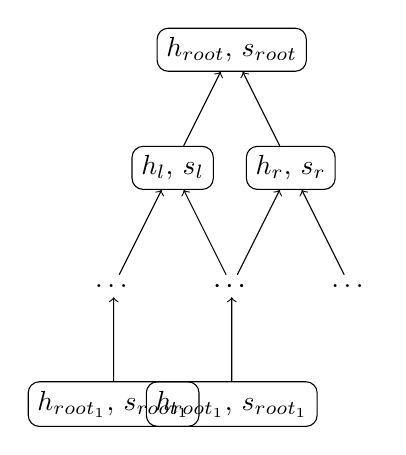
\begin{tikzpicture}
    [ edge from parent/.style={<-, draw},
      root-node/.style = {
        shape=rectangle, rounded corners,
        draw, align=center
      },
      sub-node/.style = {
        shape=rectangle, rounded corners,
        draw, align=center, fill=black!10
      },
      txt/.style = {}]
      \node [root-node] {$h_{root}$, $s_{root}$}
      child { node [root-node] {$h_l$, $s_l$}
        child { node [txt] {\ldots}
          child { node [root-node] {$h_{root_1}$, $s_{root_1}$} } }
        child { node [txt] {\ldots}
          child { node [root-node] {$h_{root_1}$, $s_{root_1}$} } } }
      child { node [root-node] {$h_r$, $s_r$}
        child { node [txt] {\ldots} }
        child { node [txt] {\ldots} } };
  \end{tikzpicture}
  \label{apx:pools:lvl2block}
  \caption{Two-level hierarchical Merkle tree for a block published by a pool
    manager}
\end{figure}

\subsubsection{General approach}

The idea is the following:

\begin{itemize}
\item Every small Educator still maintains her own small private chain
\item When a small Educator forms a block in her private chain, she sends the
  block header to a third party called \textit{pool manager} instead of
  publishing it directly to Witnesses.
\item A \textit{pool manager} collects block headers from Educators until
  total number of transactions in all Educator's blocks is more than some
  threshold $K_{min}$.
\item Then pool manager builds a sized Merkle tree over the list of received
  Educator's block headers, forming a \textit{second-level block}
  (\ref{apx:pools:lvl2block}). The header of second-level block gets published
  on the public blockchain.
\item After constructing a second-level block, pool manager sends each of the
  small Educators a path to their block headers in a second-level sized Merkle tree.
\item Having this path, each Educator can construct a publicly verifiable proof
  for any transaction in her private block by simply concatenating this path
  with a path to transaction in a first-level Merkle tree.
\end{itemize}

For every processed block header small educator pays pool manager a fee
calculated by this formula:
\begin{equation}\label{apx:pools:pools-cost-eq}
  C_{pool}(B) = \alpha_{pool} + \beta_{pub} \cdot N_{tr}(B)
\end{equation}
where $\beta_{pub}$ is a network price coefficient from
\ref{sec:priv-chain:pub-cost-eq}, and $\alpha_{pool}$ is a constant fee set by
the pool manager.

If a pool manager sets such $\alpha_{pool}$ that
$\alpha_{pool} < \alpha_{pub}$, but $\alpha_{pool} N > \alpha_{pub}$, then for
every published second-level block a pool manager gains
$\alpha_{pool} N - \alpha_{pub}$ coins, while every Educator in pool pays less
for the block header publishing then if published directly to Witnesses.
Therefore, every participant has an incentive to remain in the pool.

\subsubsection{Trustless payments to a pool manager}

TBD
